\documentclass{report}
% Include all project wide packages here.
\usepackage{fullpage}
\usepackage[style=ieee]{biblatex}
\usepackage[dutch]{babel}

\renewcommand{\familydefault}{\sfdefault}

\setmainfont[Ligatures=TeX]{Myriad Pro}
\setmathfont{Asana Math}
\setmonofont{Lucida Console}

\usepackage{titlesec, blindtext, color}
\definecolor{gray75}{gray}{0.75}
\newcommand{\hsp}{\hspace{20pt}}
\titleformat{\chapter}[hang]{\Huge\bfseries}{\thechapter\hsp\textcolor{gray75}{|}\hsp}{0pt}{\Huge\bfseries}
\renewcommand{\familydefault}{\sfdefault}
\renewcommand{\arraystretch}{1.2}
\setlength\parindent{0pt}

%For code listings
\definecolor{black}{rgb}{0,0,0}
\definecolor{browntags}{rgb}{0.65,0.1,0.1}
\definecolor{bluestrings}{rgb}{0,0,1}
\definecolor{graycomments}{rgb}{0.4,0.4,0.4}
\definecolor{redkeywords}{rgb}{1,0,0}
\definecolor{bluekeywords}{rgb}{0.13,0.13,0.8}
\definecolor{greencomments}{rgb}{0,0.5,0}
\definecolor{redstrings}{rgb}{0.9,0,0}
\definecolor{purpleidentifiers}{rgb}{0.01,0,0.01}


\lstdefinestyle{csharp}{
language=[Sharp]C,
showspaces=false,
showtabs=false,
breaklines=true,
showstringspaces=false,
breakatwhitespace=true,
escapeinside={(*@}{@*)},
columns=fullflexible,
commentstyle=\color{greencomments},
keywordstyle=\color{bluekeywords}\bfseries,
stringstyle=\color{redstrings},
identifierstyle=\color{purpleidentifiers},
basicstyle=\ttfamily\small}

\lstdefinestyle{c}{
language=C,
showspaces=false,
showtabs=false,
breaklines=true,
showstringspaces=false,
breakatwhitespace=true,
escapeinside={(*@}{@*)},
columns=fullflexible,
commentstyle=\color{greencomments},
keywordstyle=\color{bluekeywords}\bfseries,
stringstyle=\color{bluestrings},
identifierstyle=\color{purpleidentifiers}
}

\lstdefinestyle{vhdl}{
language=VHDL,
showspaces=false,
showtabs=false,
breaklines=true,
showstringspaces=false,
breakatwhitespace=true,
escapeinside={(*@}{@*)},
columns=fullflexible,
commentstyle=\color{greencomments},
keywordstyle=\color{bluekeywords}\bfseries,
stringstyle=\color{redstrings},
identifierstyle=\color{purpleidentifiers}
}

\lstdefinestyle{xaml}{
language=XML,
showspaces=false,
showtabs=false,
breaklines=true,
showstringspaces=false,
breakatwhitespace=true,
escapeinside={(*@}{@*)},
columns=fullflexible,
commentstyle=\color{greencomments},
keywordstyle=\color{redkeywords},
stringstyle=\color{bluestrings},
tagstyle=\color{browntags},
morestring=[b]",
  morecomment=[s]{<?}{?>},
  morekeywords={xmlns,version,typex:AsyncRecords,x:Arguments,x:Boolean,x:Byte,x:Char,x:Class,x:ClassAttributes,x:ClassModifier,x:Code,x:ConnectionId,x:Decimal,x:Double,x:FactoryMethod,x:FieldModifier,x:Int16,x:Int32,x:Int64,x:Key,x:Members,x:Name,x:Object,x:Property,x:Shared,x:Single,x:String,x:Subclass,x:SynchronousMode,x:TimeSpan,x:TypeArguments,x:Uid,x:Uri,x:XData,Grid.Column,Grid.ColumnSpan,Click,ClipToBounds,Content,DropDownOpened,FontSize,Foreground,Header,Height,HorizontalAlignment,HorizontalContentAlignment,IsCancel,IsDefault,IsEnabled,IsSelected,Margin,MinHeight,MinWidth,Padding,SnapsToDevicePixels,Target,TextWrapping,Title,VerticalAlignment,VerticalContentAlignment,Width,WindowStartupLocation,Binding,Mode,OneWay,xmlns:x}
}

%defaults
\lstset{
basicstyle=\ttfamily\small,
extendedchars=false,
numbers=left,
numberstyle=\ttfamily\tiny,
stepnumber=1,
tabsize=4,
numbersep=5pt
}
\addbibresource{../../library/bibliography.bib}

\title{EPO-2: Design Report - Controller}
\author{Chy Lau}

\begin{document}
\chapter{Controller}
\label{ch:controller}

\section{Werkingsprincipe}
De robot volgt na het indrukken van de reset knop een rechte lijn.
Er wordt pas naar een andere state gegaan wanneer de robot: een kruispunt, een wit oppervlak of een mijn detecteert.


Bij een kruispunt vraagt de robot welke kant hij op moet, dit is afhankelijk van de kortste route.
Het vragen en ontvangen van een signaal moet eerst worden goedgekeurd voordat de state volgt waar de robot een koers krijgt.


Bij een wit oppervlak vraagt de robot of hij klaar is met het rijden van de route.
Als dat wel het geval is, stopt de robot met rijden.
Zo niet, dan blijft de robot vooruit rijden.

Als er een mijn wordt gedetecteerd, dan wordt er doorgegeven aan de computer dat er een mijn op het wedstrijdveld is. 
Afhankelijk van de kortste route maakt de robot twee verschillende bewegingen na het detecteren van een mijn:
\begin{itemize}
\item Als de robot naar links of rechts moet bij het net bezochte kruispunt, dan rijdt hij achteruit;
\item Als de robot rechtdoor moet bij het net bezochte kruispunt, dan maakt hij een rotatie van 180$^\circ$;
\end{itemize}

De finite-state machine is bijgevoegd in de Bijlagen (Sectie \ref{sec:statemachines}, Figuur \ref{fig:fsmMain})

\begin{figure}
\centering
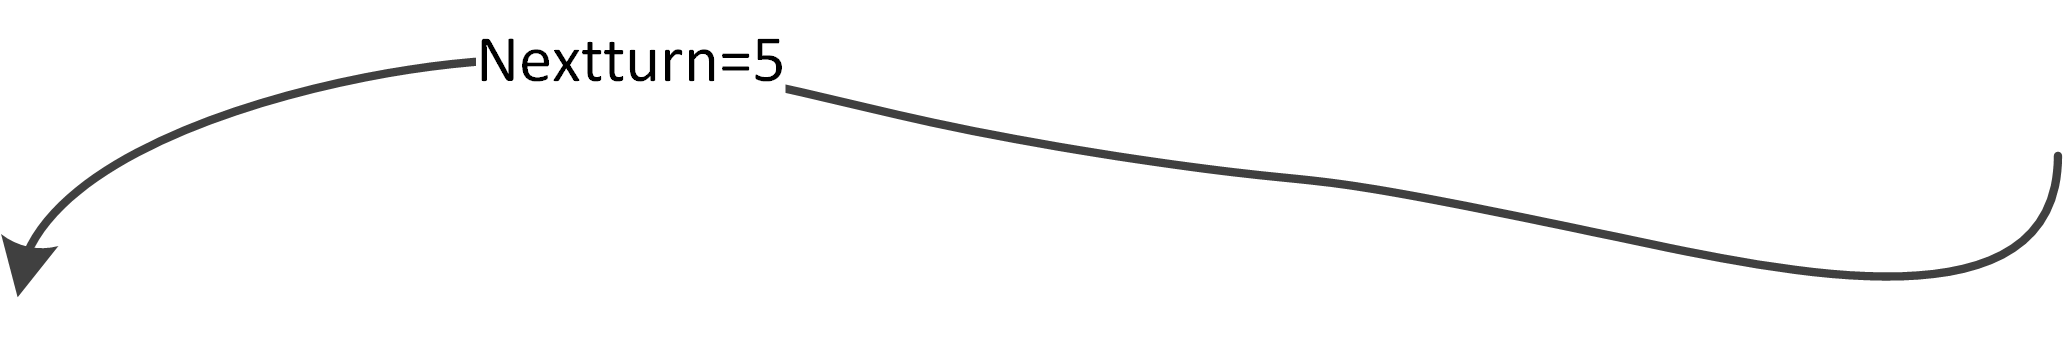
\includegraphics[scale=0.5]{../bijlagen/FSMMain.png}
\caption{De finite-state machine van de controller.}
\label{fig:fsmmain}
\end{figure}

\section{DebugID}
Om te zien of de robot alle states goed doorloopt is de DebugID ge\"{i}mplementeerd.
Iedere state is een nummer toegewezen, dat op het 7-segment display wordt weergegeven.
Stel dat de robot de verkeerde beweging maakt tijdens het rijden op het wedstrijdveld, dan kan er gekeken worden naar welke state de robot is gegaan tijdens het maken van de verkeerde beweging.
Dit maakt het oplossen van problemen eenvoudiger en sneller.


\section{FSM-states}

\subsection{Delay-state}
In de delay-state staat een delay-counter die ervoor zorgt dat er tijdens de delay geen signaal naar de computer wordt gestuurd.
Dit is handig, want de robot zal bij een rechte lijn niet steeds aan de computer vragen waar hij heen moet.
De robot zal daardoor vloeiend rechtdoor rijden in plaats van een stutter beweging maken.
Er is voor de delay-counter een bepaalde waarde gekozen en zal na iedere opgaande klokflank met 1 verminderen.
Als de delay-counter dan op 0 komt te staan, wordt er een nieuwe state gevraagd.
In principe zorgt de delay-state ervoor dat het interval van het vragen van een nieuwe state wordt vergroot.


\subsection{Followline-state}
De main state waar de robot in begint nadat de reset wordt ingedrukt is Followline.
De robot volgt de lijn op het wedstrijdveld en als er afwijkingen zijn, wordt de baan door middel van de sensoren gecorrigeerd.
Tijdens het volgen van de lijn kunnen de volgende states voorkomen: 
\begin{itemize}
\item De robot staat op het kruispunt en wacht op het volgende commando;
\item De robot ziet een witte lijn en vraagt of dit het einde is van de route;
\item De robot detecteert een mijn en maakt een draai van 180$^\circ$ of hij rijdt achteruit totdat de sensoren een kruispunt detecteren;
\end{itemize}

\subsection{Callforinput-state}
Wanneer de robot bij een kruising komt (de sensoren registeren alle drie zwart) en de delay-counter is gelijk aan nul, dan gaat de robot naar de Callforinput-state.
In deze state wordt er aan de computer gevraagd wat de robot moet doen.
Als het vragen naar een input aangekomen en goedgekeurd is, dan wacht de robot op een commando.
Gaat deze stap goed, dan volgt de Processnextturn-state, zo niet, dan vraagt de robot weer aan de computer om een input.

\subsection{Processnextturn-state}
In de Processnextturn-state wordt de ontvangen input ge\"{e}valueerd.
Afhankelijk van de input gaat de robot naar de volgende states:
\begin{itemize}
\item Leftturn-state: de robot maakt een bocht naar links, totdat de sensoren een rechte lijn detecteren, dan volgt de robot de rechte lijn;
\item Followline-state: de robot gaat in deze state wanneer er een direct commando is gegeven om de rechte lijn te volgen of wanneer de robot klaar is met maken van een bocht/draaiing;
\item Rightturn-state: analoog aan de Leftturn-state;
\item Fullturn-state: de robot maakt een draai van 180$^\circ$, daarna volgt hij een rechte lijn;
\item Back-state: de robot rijdt achteruit totdat de sensor bij het kruispunt is en maakt een bocht naar links of rechts;
\item Callforinput-state: er wordt gevraagd aan de computer wat het volgende commando is;
Dit leidt ertoe dat de robot steeds blijft vragen wat het volgende commando is, oftewel het resultaat is dat de robot stopt.
Bovendien wordt de UART-receiver gereset;
\end{itemize} 

\subsection{Sendmine-state}
De robot gaat naar de Sendmine-state wanneer hij tijdens het volgen van een lijn een mijn detecteert.
In deze state stop de robot met rijden en wordt er aan de computer doorgegeven dat er een mijn ligt.
Als dat is goedgekeurd, gaat de robot afhankelijk van de kortste route in de Followline-state of Back-state.

\subsection{Arewedone-state}
De Arewedone-state volgt na het detecteren van een wit oppervlak.
Er wordt gevraagd of het bepaalde punt het einde is van de route.
Als dat zo is, volgt de Done-state en stopt de robot.
Zo niet, dan volgt de Followline-state.
Bovendien is er in de Done-state nog een mogelijkheid om de robot de laten rijden nadat hij stilstaat.
\end{document}